\chapter{त्रिविम रसायन का गहन अध्ययन}\label{ch:b1:stereochemistry-in-depth}

विलायती जीरे के कुछ दाने मसलिए, फिर पुदीने की एक पत्ती: दो बिल्कुल
अलग गंधें। दोनों की मुख्य गंधदायक वस्तु कार्वोन, \ce{C10H14O}, है --- वही परमाणु,
उसी क्रम में जुड़े हुए --- पर दोनों कार्वोन एक-दूसरे के दर्पण-प्रतिबिंब हैं, जैसे
बायाँ हाथ दाएँ हाथ का, और नाक के ग्राही, जो स्वयं दर्पण-असममित अणुओं से
बने हैं, उन्हें अलग-अलग पहचान लेते हैं। औषधियाँ, सुगंध-स्वाद और जीवन के अणु
सभी तीन विमाओं में बने हैं, और जो संरचना सूत्र तीसरी विमा की उपेक्षा करता है
वह आधी कहानी छोड़ देता है। यह अध्याय अणुओं को अंतरिक्ष में खींचने, हर
व्यवस्था को बिना किसी संदिग्धता के नाम देने, अणुओं द्वारा निरंतर किए जाने वाले
घूर्णनों का अनुसरण करने, और उस एकमात्र भौतिक गुण को मापने के उपकरण देता है
जो दर्पण-प्रतिबिंबों में भेद करता है।

\begin{recall}
विद्यालय के खंड (कक्षा 12) ने \omterm{def:b1:stereochemistry-in-depth:stereocentre}{किरैल} अणुओं, असममित कार्बन, \omterm{def:b1:stereochemistry-in-depth:enantiomers}{प्रतिबिंबरूपियों},
$Z$/$E$ समावयवियों और एथेन के \omterm{def:b1:stereochemistry-in-depth:isomers}{संरूपणों} का परिचय दिया था। कार्बन के चारों ओर
चार आबंधों की चतुष्फलकीय व्यवस्था और एकल तथा द्वि-आबंधों का
$\sigma$/$\pi$ वर्णन \cref{ch:b1:lewis-resonance-vsepr} से आते हैं।
\end{recall}

\begin{omfigure}
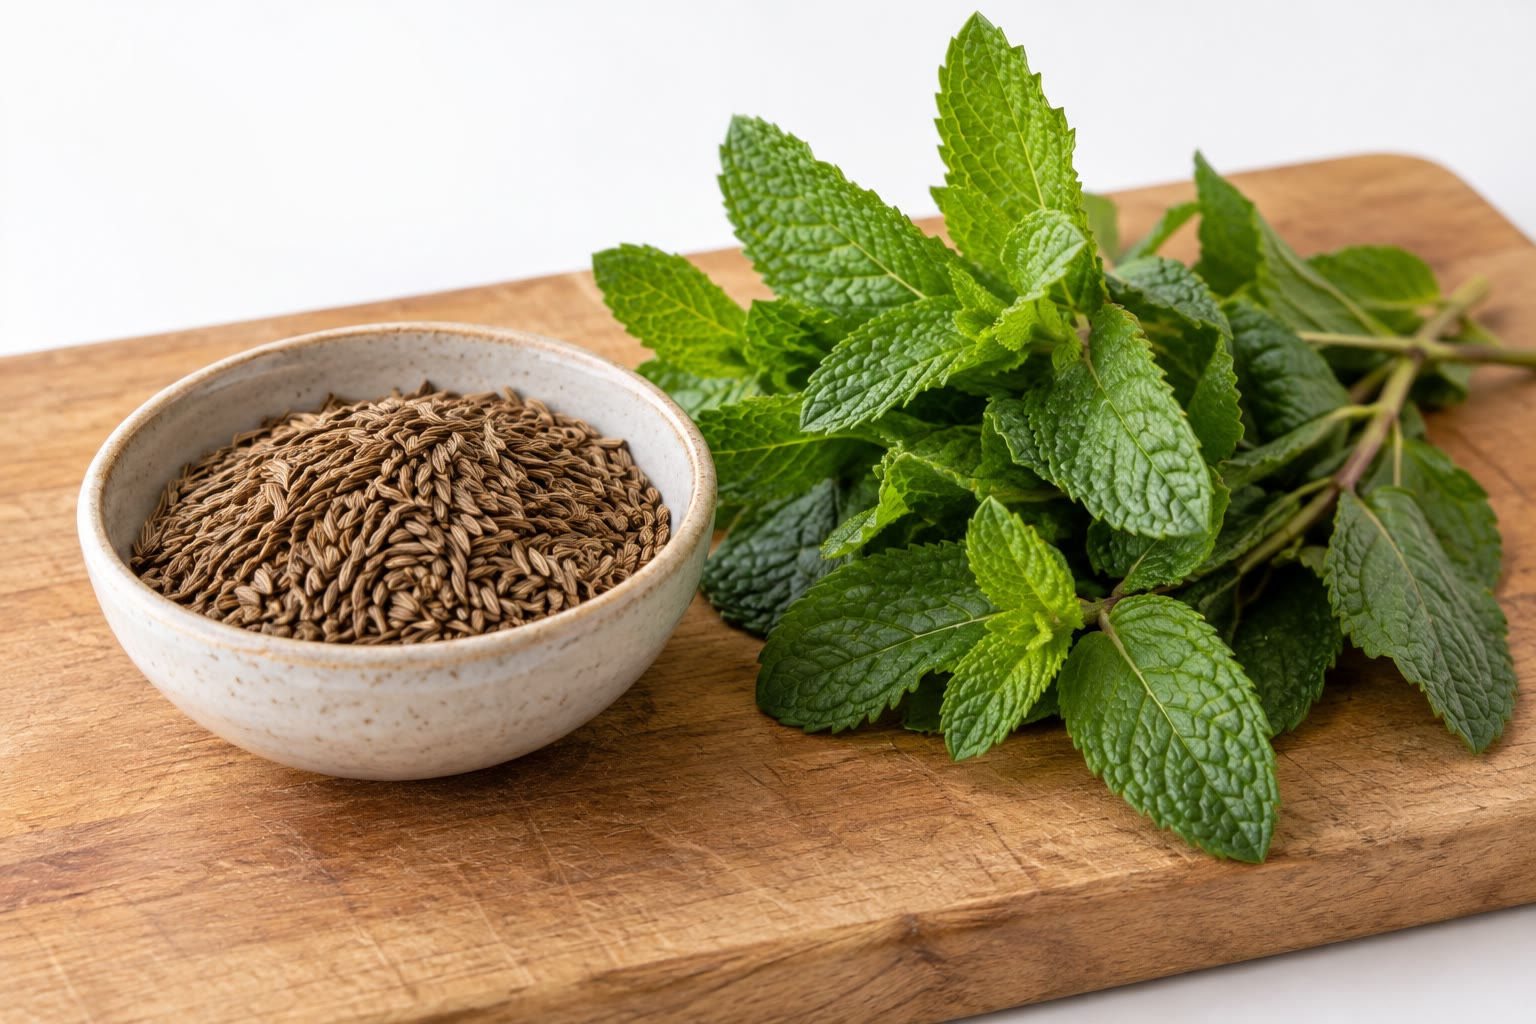
\includegraphics[width=0.55\linewidth]{images/book2/ai/b1-16-caraway-mint.jpg}

{\small विलायती जीरे के दाने और पुदीने की पत्तियाँ। विलायती जीरे की गंध मुख्यतः
\cip{S}-कार्वोन से आती है, पुदीने की उसके दर्पण-प्रतिबिंब \cip{R}-कार्वोन से।}
\end{omfigure}

\section{समावयवी और निरूपण}

\begin{definition}[संरचना, विन्यास, संरूपण]\label{def:b1:stereochemistry-in-depth:isomers}
समान सूत्र वाले दो यौगिक जिनके परमाणु भिन्न क्रम में जुड़े हों,
\emph{संरचनात्मक समावयवी}\index{संरचनात्मक समावयवी} हैं।
समान संरचना वाले यौगिक जिनके परमाणु केवल अंतरिक्ष में अपनी व्यवस्था में भिन्न हों,
\emph{त्रिविम समावयवी}\index{त्रिविम समावयवी} हैं। जिस
व्यवस्था को केवल आबंध तोड़कर ही बदला जा सकता है, वह किसी त्रिविम समावयवी का
\emph{विन्यास}\index{विन्यास} है; एकल आबंधों के परितः घूर्णन से, बिना कोई आबंध तोड़े,
प्राप्त व्यवस्था एक \emph{संरूपण}\index{संरूपण} है।
\end{definition}

कमरे के ताप पर, एकल आबंधों के परितः घूर्णन प्रति सेकंड अरबों बार होते हैं:
\omterm{def:b1:stereochemistry-in-depth:isomers}{संरूपण} एक-दूसरे में बदलते रहते हैं और उन्हें पृथक नहीं किया जा सकता, जबकि
\omterm{def:b1:stereochemistry-in-depth:isomers}{विन्यास} स्थायी होते हैं और अलग-अलग यौगिक देते हैं।

\begin{definition}[निरूपण]\label{def:b1:stereochemistry-in-depth:representations}
\emph{क्रैम निरूपण}\index{क्रैम निरूपण} में दो आबंध
पृष्ठ के तल में खींचे जाते हैं, एक ठोस फन्नी पाठक की ओर संकेत करती है
और एक धारीदार फन्नी उससे दूर। \emph{न्यूमैन प्रक्षेप}\index{न्यूमैन प्रक्षेप}
किसी अणु को एक C--C आबंध की दिशा में देखता है: सामने वाला कार्बन एक
बिंदु है जहाँ उसके तीन अन्य आबंध मिलते हैं, पीछे वाला कार्बन एक वृत्त जिसकी
परिधि से उसके आबंध निकलते हैं। \emph{फ़िशर प्रक्षेप}\index{फ़िशर प्रक्षेप} में
कार्बन शृंखला ऊर्ध्वाधर होती है, क्षैतिज आबंध पाठक की ओर संकेत करते हैं
और ऊर्ध्वाधर आबंध उससे दूर; हर क्रॉस एक त्रिविमजनक कार्बन है।
\end{definition}

\begin{omfigure}
\begin{tikzpicture}[font=\small]
  % staggered and eclipsed ethane, Newman
  \pic (s) at (0,0) {omnewman={90}{30}};
  \foreach \k in {1,2,3} { \node at (s-f\k) {H}; \node at (s-b\k) {H}; }
  \node at (0,-1.9) {सांतरित};
  \pic (e) at (3.6,0) {omnewman={90}{108}};
  \foreach \k in {1,2,3} { \node at (e-f\k) {H}; }
  \foreach \k in {1,2,3} { \node[font=\scriptsize, black!60] at ($(e-b\k)!-0.12!(e-c)$) {H}; }
  \node at (3.6,-1.9) {ग्रसित};
  % Fischer projection of (R)-lactic acid
  \begin{scope}[xshift=7.6cm]
    \draw[thick] (-0.9,0) -- (0.9,0) (0,-0.9) -- (0,0.9);
    \node[above] at (0,0.9) {\ce{COOH}};
    \node[below] at (0,-0.9) {\ce{CH3}};
    \node[left] at (-0.9,0) {H};
    \node[right] at (0.9,0) {OH};
    \node at (0,-1.9) {फ़िशर};
  \end{scope}
  % Cram of the same
  \begin{scope}[xshift=11.0cm]
    \node at (0,0) {\chemfig{C(-[2]COOH)(-[:210]H_3C)(<:[:-12]OH)(<[:-55]H)}};
    \node at (0,-1.9) {क्रैम};
  \end{scope}
\end{tikzpicture}

{\small बाएँ: एथेन के C--C आबंध की दिशा में उसके \omterm{def:b1:stereochemistry-in-depth:representations}{न्यूमैन प्रक्षेप}, सांतरित
(पीछे के आबंध सामने वालों के बीच में) और ग्रसित (पीछे के आबंध सामने वालों के
पीछे छिपे, थोड़ा हटाकर खींचे गए)। दाएँ: वही अणु,
\cip{R}-लैक्टिक अम्ल, \omterm{def:b1:stereochemistry-in-depth:representations}{फ़िशर प्रक्षेप} के रूप में और \omterm{def:b1:stereochemistry-in-depth:representations}{क्रैम निरूपण} में
(फ़िशर क्रॉस के ऊर्ध्वाधर आबंध पाठक से दूर संकेत करते हैं,
क्षैतिज आबंध पाठक की ओर)।}
\end{omfigure}

\begin{method}[क्रैम से न्यूमैन तक]\label{met:b1:stereochemistry-in-depth:newman-from-cram}
\begin{enumerate}
  \item वह आबंध चुनिए जिसकी दिशा में देखना है, और उसका वह सिरा जो आँख के पास है।
  \item सामने वाले कार्बन के तीन आबंध केंद्र से खींचिए,
        उनका क्रम (दक्षिणावर्त या वामावर्त) वैसा ही रखते हुए जैसा
        आँख से दिखता है।
  \item पीछे वाले कार्बन के आबंध वृत्त से खींचिए, उनका क्रम वैसा ही रखते हुए जैसा
        उसी ओर से दिखता है।
  \item जाँच: पीछे वाले कार्बन को $60^\circ$ घुमाने पर
        सांतरित से ग्रसित पर पहुँचते हैं; $120^\circ$ घुमाने पर, एक \omterm{def:b1:stereochemistry-in-depth:conformations}{सांतरित
        संरूपण} से अगले पर।
\end{enumerate}
\end{method}

\section{विन्यास: CIP नियम}

\begin{definition}[CIP नियम, वर्णक]\label{def:b1:stereochemistry-in-depth:cip}
\emph{CIP नियम}\index{CIP नियम} (कान--इंगोल्ड--प्रेलॉग) किसी \omterm{def:b1:stereochemistry-in-depth:stereocentre}{त्रिविमजनक केंद्र} के
चार प्रतिस्थापियों को क्रम देते हैं: अधिक परमाणु क्रमांक पहले; बराबरी
होने पर, अगले जुड़े परमाणुओं के समुच्चयों की तुलना कीजिए, और इसी तरह बाहर की ओर; एक
द्वि-आबंध दो प्रतिरूपित परमाणुओं से दो एकल आबंधों के रूप में गिना जाता है। जब
निम्नतम क्रम का प्रतिस्थापी आँख से दूर संकेत करे, तब अनुक्रम
$1 \to 2 \to 3$ का दक्षिणावर्त घूमना वर्णक \cip{R} परिभाषित करता है, और
वामावर्त \cip{S}। ऐसे द्वि-आबंध के लिए जिसके हर कार्बन पर दो प्रतिस्थापी हों,
\cip{Z} का अर्थ है कि उच्चतर क्रम वाले दोनों एक ही ओर हैं, और
\cip{E} कि विपरीत ओर।
\end{definition}

\begin{method}[\texorpdfstring{\cip{R}}{(R)} या \texorpdfstring{\cip{S}}{(S)} निर्धारित करना]\label{met:b1:stereochemistry-in-depth:cip}
\begin{enumerate}
  \item चारों प्रतिस्थापियों को \omterm{def:b1:stereochemistry-in-depth:cip}{CIP नियमों} से क्रम दीजिए।
  \item यदि निम्नतम क्रम वाला आपसे दूर संकेत करता है (धारीदार फन्नी, या
        \omterm{def:b1:stereochemistry-in-depth:representations}{फ़िशर प्रक्षेप} का ऊर्ध्वाधर आबंध), तो
        $1 \to 2 \to 3$ का घुमाव सीधे पढ़िए।
  \item यदि वह आपकी ओर संकेत करता है (ठोस फन्नी, क्षैतिज फ़िशर आबंध),
        तो घुमाव पढ़िए और वर्णक उलट दीजिए।
  \item किन्हीं दो प्रतिस्थापियों की अदला-बदली वर्णक को उलट देती है: एक त्वरित
        जाँच।
\end{enumerate}
लैक्टिक अम्ल में $\ce{OH} > \ce{COOH} > \ce{CH3} > \ce{H}$ (O; फिर C(O,O,O)
C(H,H,H) से आगे है)। ऊपर के \omterm{def:b1:stereochemistry-in-depth:representations}{फ़िशर प्रक्षेप} में H क्षैतिज है
(हमारी ओर) और $\ce{OH} \to \ce{COOH} \to \ce{CH3}$ वामावर्त घूमता है:
उलटने पर, केंद्र \cip{R} है।
\end{method}

\section{किरैलता और उसके परिणाम}

\begin{definition}[त्रिविमजनक केंद्र, किरैलता]\label{def:b1:stereochemistry-in-depth:stereocentre}
कोई वस्तु \emph{किरैल}\index{किरैल} है यदि उसे उसके
दर्पण-प्रतिबिंब पर अध्यारोपित न किया जा सके, अन्यथा \emph{अकिरैल}\index{अकिरैल}; यह गुण
\emph{किरैलता}\index{किरैलता} है। \emph{त्रिविमजनक
केंद्र}\index{त्रिविमजनक केंद्र} वह परमाणु है जिस पर दो प्रतिस्थापियों की
अदला-बदली से एक \omterm{def:b1:stereochemistry-in-depth:isomers}{त्रिविम समावयवी} मिलता है; चार भिन्न प्रतिस्थापियों वाला
चतुष्फलकीय कार्बन ऐसा ही एक केंद्र है।
\end{definition}

सममिति-तल या सममिति-केंद्र वाला अणु \omterm{def:b1:stereochemistry-in-depth:stereocentre}{अकिरैल} होता है;
जिस अणु में दोनों में से कोई न हो, वह व्यवहार में \omterm{def:b1:stereochemistry-in-depth:stereocentre}{किरैल} होता है। सममिति संक्रियाओं
के रूप में यथार्थ कसौटी तृतीय वर्ष के खंड में दी गई है।

\begin{definition}[प्रतिबिंबरूपी, अप्रतिबिंबरूपी, मेसो यौगिक, रेसेमिक मिश्रण]\label{def:b1:stereochemistry-in-depth:enantiomers}
जो दो \omterm{def:b1:stereochemistry-in-depth:isomers}{त्रिविम समावयवी} एक-दूसरे के दर्पण-प्रतिबिंब हों, वे
\emph{प्रतिबिंबरूपी}\index{प्रतिबिंबरूपी} हैं; जो \omterm{def:b1:stereochemistry-in-depth:isomers}{त्रिविम समावयवी} ऐसे न हों, वे
\emph{अप्रतिबिंबरूपी}\index{अप्रतिबिंबरूपी} हैं। \emph{मेसो
यौगिक}\index{मेसो यौगिक} में \omterm{def:b1:stereochemistry-in-depth:stereocentre}{त्रिविमजनक केंद्र} होते हैं पर वह \omterm{def:b1:stereochemistry-in-depth:stereocentre}{अकिरैल} होता है।
दो प्रतिबिंबरूपियों का सम-मोलर मिश्रण \emph{रेसेमिक
मिश्रण}\index{रेसेमिक मिश्रण} है।
\end{definition}

\begin{proposition}[त्रिविम समावयवियों की संख्या]\label{prop:b1:stereochemistry-in-depth:max-stereoisomers}
$n$ \omterm{def:b1:stereochemistry-in-depth:stereocentre}{त्रिविमजनक केंद्रों} (और किसी अन्य त्रिविमजनक इकाई के बिना) वाले अणु के
अधिक से अधिक $2^n$ \omterm{def:b1:stereochemistry-in-depth:isomers}{त्रिविम समावयवी} होते हैं, \omterm{def:b1:stereochemistry-in-depth:enantiomers}{प्रतिबिंबरूपियों} के अधिक से अधिक
$2^{n-1}$ युग्मों में; मेसो रूप यह संख्या घटा देते हैं।
\end{proposition}

\begin{proof}
हर केंद्र स्वतंत्र रूप से \cip{R} या \cip{S} है: $2^n$ संयोजन।
दर्पण-प्रतिबिंब हर वर्णक को बदल देता है, इसलिए संयोजन जोड़ियों में
\omterm{def:b1:stereochemistry-in-depth:enantiomers}{प्रतिबिंबरूपी} बनाते हैं, $2^{n-1}$ युग्म। यदि कोई संयोजन अणु के घूर्णन के बाद
स्वयं अपना दर्पण-प्रतिबिंब हो (एक मेसो रूप), तो उसका युग्म सिमटकर
एक ही यौगिक रह जाता है।
\end{proof}

टार्टरिक अम्ल, \ce{HOOC-CH(OH)-CH(OH)-COOH}, में दो तुल्य केंद्र हैं:
\cip{R,R} और \cip{S,S} \omterm{def:b1:stereochemistry-in-depth:enantiomers}{प्रतिबिंबरूपी} हैं, जबकि \cip{R,S} में दोनों कार्बनों के बीच
एक दर्पण-तल है और वह मेसो है: तीन \omterm{def:b1:stereochemistry-in-depth:isomers}{त्रिविम समावयवी}, चार नहीं।

\begin{proposition}[प्रतिबिंबरूपियों के गुण]\label{prop:b1:stereochemistry-in-depth:enantiomer-properties}
दो \omterm{def:b1:stereochemistry-in-depth:enantiomers}{प्रतिबिंबरूपियों} के गलनांक और क्वथनांक, \omterm{def:b1:stereochemistry-in-depth:stereocentre}{अकिरैल} विलायकों में \omterm{def:b1:precipitation:solubility}{विलेयताएँ},
स्पेक्ट्रम और \omterm{def:b1:stereochemistry-in-depth:stereocentre}{अकिरैल} अभिकर्मकों के प्रति अभिक्रियाशीलता समान होते हैं;
वे ध्रुवित प्रकाश पर अपनी क्रिया में और अन्य \omterm{def:b1:stereochemistry-in-depth:stereocentre}{किरैल} अणुओं के साथ अपनी
अन्योन्यक्रियाओं में भिन्न होते हैं। \omterm{def:b1:stereochemistry-in-depth:enantiomers}{अप्रतिबिंबरूपी} अपने सभी गुणों में
भिन्न होते हैं।
\end{proposition}

\begin{proof}
हर वह गुण जो केवल अणु के भीतर की, या अणु और \omterm{def:b1:stereochemistry-in-depth:stereocentre}{अकिरैल} साथियों के बीच की,
दूरियों और कोणों पर निर्भर करता है, किसी वस्तु और उसके दर्पण-प्रतिबिंब के लिए
समान होता है, क्योंकि परावर्तन दूरियों और कोणों को संरक्षित रखता है।
एक \omterm{def:b1:stereochemistry-in-depth:stereocentre}{किरैल} साथी (एक ग्राही, एक \omterm{def:b1:stereochemistry-in-depth:stereocentre}{किरैल} अभिकर्मक, आगे वर्णित ध्रुवित प्रकाश का
सर्पिल पथ) ऐसे जोड़े बनाता है जो \omterm{def:b1:stereochemistry-in-depth:enantiomers}{अप्रतिबिंबरूपी} होते हैं, अब दर्पण-प्रतिबिंब नहीं,
और इसलिए भिन्न होते हैं। \omterm{def:b1:stereochemistry-in-depth:enantiomers}{अप्रतिबिंबरूपी} किसी भी परावर्तन से
संबंधित नहीं हैं: उनकी आंतरिक दूरियाँ भिन्न होती हैं।
\end{proof}

\begin{omfigure}
\begin{tikzpicture}[font=\small, line join=round]
  \foreach \dx/\kind/\lab in {0/1/{\cip{R}-कार्वोन (पुदीना)}, 5.2/0/{\cip{S}-कार्वोन (विलायती जीरा)}} {
  \begin{scope}[xshift=\dx cm]
    \coordinate (c1) at (0,1); \coordinate (c2) at (0.87,0.5);
    \coordinate (c3) at (0.87,-0.5); \coordinate (c4) at (0,-1);
    \coordinate (c5) at (-0.87,-0.5); \coordinate (c6) at (-0.87,0.5);
    \draw[thick] (c1) -- (c2) -- (c3) -- (c4) -- (c5) -- (c6) -- cycle;
    \draw[thick] ($(c2)!0.15!(c3)+(-0.12,0)$) -- ($(c3)!0.15!(c2)+(-0.12,0)$);
    \draw[thick] (c1) -- ++(0,0.7) node[above] {O};
    \draw[thick] ($(c1)+(0.1,0)$) -- ++(0,0.62);
    \draw[thick] (c2) -- ++(0.75,0.43) node[right] {\ce{CH3}};
    \coordinate (q) at ($(c5)+(-0.75,-0.43)$);
    \ifnum\kind=1
      \fill (c5) -- ($(q)+(0.06,-0.1)$) -- ($(q)+(-0.06,0.1)$) -- cycle;
    \else
      \foreach \t in {0.15,0.3,0.45,0.6,0.75,0.9}
        \draw ($(c5)!\t!(q)+(\t*0.06,-\t*0.1)$) -- ($(c5)!\t!(q)+(-\t*0.06,\t*0.1)$);
    \fi
    \draw[thick] (q) -- ++(-0.6,0.5) node[above] {\ce{CH2}};
    \draw[thick] ($(q)+(0.08,0.06)$) -- ++(-0.6,0.5);
    \draw[thick] (q) -- ++(0,-0.75) node[below] {\ce{CH3}};
    \node[font=\scriptsize] at ($(c5)+(0.35,0.12)$) {5};
    \node at (0,-2.85) {\lab};
  \end{scope}}
\end{tikzpicture}

{\small दोनों कार्वोन, एक ही कंकाल पर खींचे गए: C5 पर आइसोप्रोपेनिल समूह
एक में पाठक की ओर (ठोस फन्नी) और दूसरे में पाठक से दूर
(धारीदार फन्नी) संकेत करता है, C5 का हाइड्रोजन (खींचा नहीं गया) विपरीत
ओर। वे एक-दूसरे के दर्पण-प्रतिबिंब हैं: \omterm{def:b1:stereochemistry-in-depth:enantiomers}{प्रतिबिंबरूपी}
(\cref{exo:b1:stereochemistry-in-depth:4})।}
\end{omfigure}

\begin{history}[एक चतुष्फलकीय कार्बन]
\begin{minipage}[t]{0.2\linewidth}\vspace{0pt}
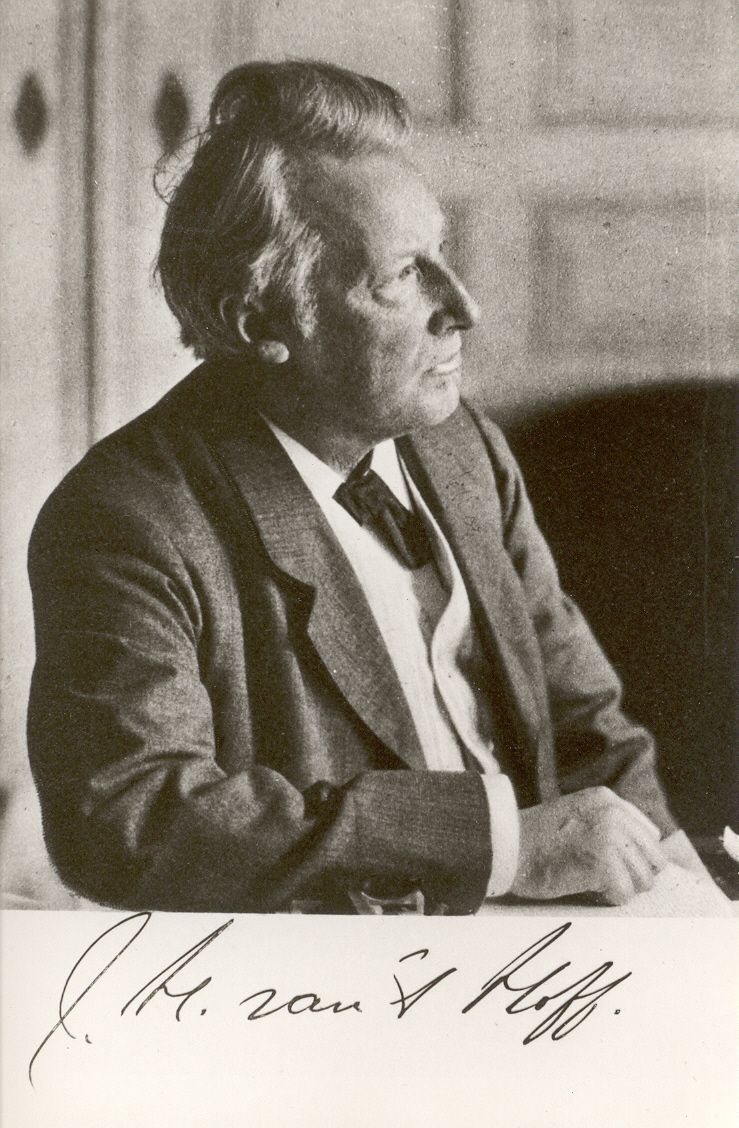
\includegraphics[width=\linewidth]{images/book2/van-t-hoff.jpg}
\end{minipage}\hfill
\begin{minipage}[t]{0.76\linewidth}\vspace{0pt}
याकोबस हेंड्रिकस वांट हॉफ़ ने, एक युवा रसायनज्ञ के रूप में, यह प्रस्ताव रखा कि
कार्बन परमाणु के चार आबंध एक चतुष्फलक के कोनों की ओर संकेत करते हैं। चार भिन्न
प्रतिस्थापियों वाला कार्बन तब दो दर्पण-प्रतिबिंब व्यवस्थाओं के रूप में
अस्तित्व में होता है, जिससे यह स्पष्ट हुआ कि कुछ यौगिक दो रूपों में क्यों मिलते हैं जो
केवल ध्रुवित प्रकाश को घुमाने के ढंग में भिन्न होते हैं। यह विचार इस अध्याय के हर
चित्र का आरंभ-बिंदु है।
(छायाचित्र 1911 में प्रकाशित, सार्वजनिक अधिकार-क्षेत्र, विकिमीडिया कॉमन्स।)
\end{minipage}
\end{history}

\section{संरूपण}

\begin{definition}[मरोड़ कोण और संरूपण]\label{def:b1:stereochemistry-in-depth:conformations}
चार परमाणुओं A--B--C--D के लिए, B--C के परितः \emph{मरोड़ कोण}\index{मरोड़ कोण}
$\theta$ तलों ABC और BCD के बीच का कोण है, जिसे B--C की दिशा में
\omterm{def:b1:stereochemistry-in-depth:representations}{न्यूमैन प्रक्षेप} पर पढ़ा जाता है। कोई \omterm{def:b1:stereochemistry-in-depth:isomers}{संरूपण} \emph{ग्रसित
संरूपण}\index{ग्रसित संरूपण} है जब सामने और पीछे के कार्बनों के आबंध
प्रक्षेप में संरेखित हों, और \emph{सांतरित
संरूपण}\index{सांतरित संरूपण} जब वे बारी-बारी से हों।
ब्यूटेन में, C2--C3 की दिशा में देखने पर, वह सांतरित \omterm{def:b1:stereochemistry-in-depth:isomers}{संरूपण} जिसमें दोनों
मेथिल समूह $180^\circ$ पर हों, \emph{प्रति संरूपण}\index{प्रति संरूपण} है,
और $\pm 60^\circ$ वाले \emph{गाउश
संरूपण}\index{गाउश संरूपण} हैं। साइक्लोहेक्सेन में,
तनाव-मुक्त सिकुड़ा हुआ वलय \emph{कुर्सी}\index{कुर्सी} है; हर कार्बन
एक \emph{अक्षीय}\index{अक्षीय} आबंध रखता है, जो वलय के
अक्ष के समांतर है, और एक \emph{विषुवतीय}\index{विषुवतीय} आबंध, जो लगभग
वलय के माध्य तल में है। \emph{वलय पलटन}\index{वलय पलटन} एक
कुर्सी को दूसरी में बदल देता है, हर अक्षीय आबंध विषुवतीय बन जाता है और
विषुवतीय अक्षीय।
\end{definition}

\begin{omfigure}
\begin{tikzpicture}
\begin{axis}[
  width=0.82\linewidth, height=5.8cm, xmin=0, xmax=360, ymin=0, ymax=21,
  legend style={font=\scriptsize, draw=none, at={(0.5,0.62)}, anchor=center},
  axis x line=bottom, axis y line=left, xlabel={मरोड़ कोण $\theta$ (डिग्री)},
  ylabel={ऊर्जा (kJ/mol)}, xtick={0,60,120,180,240,300,360},
  tick label style={font=\small}, label style={font=\small}]
\addplot[omDef, very thick] table[x=theta, y=butane] {figdata/out/bachelor-1-butane-torsion.dat};
\addplot[omProp, thick, dashed] table[x=theta, y=ethane] {figdata/out/bachelor-1-butane-torsion.dat};
\node[font=\scriptsize, anchor=south west] at (axis cs:0,18.4) {सम};
\node[font=\scriptsize, anchor=south] at (axis cs:62,18.4) {गाउश};
\node[font=\scriptsize, anchor=south] at (axis cs:120,18.4) {ग्रसित};
\node[font=\scriptsize, anchor=south] at (axis cs:180,18.4) {प्रति};
\node[font=\scriptsize, anchor=south] at (axis cs:240,18.4) {ग्रसित};
\node[font=\scriptsize, anchor=south] at (axis cs:298,18.4) {गाउश};
\node[font=\scriptsize, anchor=south east] at (axis cs:360,18.4) {सम};
\legend{ब्यूटेन, एथेन}
\end{axis}
\end{tikzpicture}

{\small ब्यूटेन की उसके केंद्रीय आबंध के परितः मरोड़ ऊर्जा (ठोस रेखा; $\theta
= 0$ जब मेथिल समूह एक-दूसरे को ग्रसित करते हैं) और एथेन की (धराशायी रेखा),
प्रायोगिक मरोड़ विभवों से परिकलित। एथेन: अवरोध
\qty{12.2}{kJ/mol}। ब्यूटेन: प्रति सबसे स्थायी; गाउश \qty{2.8}{kJ/mol}
ऊँचा, $\theta = 62^\circ$ पर; अवरोध \qty{15.2}{kJ/mol} (मेथिल द्वारा
हाइड्रोजन का ग्रसन) और \qty{16.5}{kJ/mol} (मेथिल द्वारा मेथिल का ग्रसन)।}
% ledger: rot:ethane-V3, rot:butane-V1, rot:butane-V2, rot:butane-V3, rot:butane-V4, rot:butane-V5, rot:butane-V6 (curves in figdata/bachelor-1/butane-torsion.py)
\end{omfigure}

संघट्टों में उपलब्ध ऊष्मीय ऊर्जा की तुलना में अवरोध छोटे हैं
(कमरे के ताप पर $RT = \qty{2.5}{kJ/mol}$, और वितरण की पूँछ में
कहीं अधिक, \cref{ch:b1:elementary-steps}): घूर्णन
तीव्र है, और ब्यूटेन प्रति और गाउश अणुओं का ऐसा मिश्रण है जिसे
पृथक नहीं किया जा सकता।

\begin{method}[कुर्सी खींचना]\label{met:b1:stereochemistry-in-depth:draw-chair}
\begin{enumerate}
  \item दाईं ओर थोड़ी नीचे झुकी हुई दो समांतर रेखाएँ खींचिए,
        एक-दूसरे से खिसकी हुई; छह-सदस्यीय वलय बंद करने के लिए उनके सिरों को
        बाईं ओर एक V से और दाईं ओर एक उलटे V से जोड़िए।
  \item \omterm{def:b1:stereochemistry-in-depth:conformations}{अक्षीय} आबंध ऊर्ध्वाधर होते हैं: ऊपर की ओर उठे कार्बनों पर ऊपर, नीचे की ओर
        झुके कार्बनों पर नीचे, वलय के चारों ओर बारी-बारी से।
  \item \omterm{def:b1:stereochemistry-in-depth:conformations}{विषुवतीय} आबंध एक स्थान छोड़कर अगले वलय-आबंधों के समांतर होते हैं, और
        बाहर की ओर संकेत करते हैं।
  \item वलय पलटने के लिए दूसरी \omterm{def:b1:stereochemistry-in-depth:conformations}{कुर्सी} खींचिए; जो प्रतिस्थापी एक में \omterm{def:b1:stereochemistry-in-depth:conformations}{अक्षीय} है
        वह दूसरी में \omterm{def:b1:stereochemistry-in-depth:conformations}{विषुवतीय} है।
\end{enumerate}
\end{method}

\begin{omfigure}
\begin{tikzpicture}[font=\small]
  \pic (a) at (0,0) {omchair};
  \foreach \k in {1,2,3,4,5,6} \draw[omProp, thick] (a-c\k) -- (a-a\k);
  \foreach \k in {1,2,3,4,5,6} \draw[omDef, thick] (a-c\k) -- (a-e\k);
  \node[omProp, anchor=south] at (a-a3) {अक्षीय};
  \node[omDef, anchor=north] at (a-e5) {विषुवतीय};
  \begin{scope}[xshift=4.9cm]
    \pic (b) at (0,0) {omchair};
    \draw[thick] (b-c1) -- (b-e1) node[right] {\ce{CH3}};
    \draw[thick] (b-c1) -- (b-a1) node[above] {H};
    \node at (0,-1.5) {विषुवतीय \ce{CH3}};
  \end{scope}
  \draw[<->, thick] (8.1,0) -- (8.8,0) node[midway, above] {\scriptsize पलटन};
  \begin{scope}[xshift=10.45cm]
    \pic (c) at (0,0) {omchairflip};
    \draw[thick] (c-c4) -- (c-a4) node[below] {\ce{CH3}};
    \draw[thick] (c-c4) -- (c-e4) node[right] {H};
    \node at (0,-1.5) {अक्षीय \ce{CH3}};
  \end{scope}
\end{tikzpicture}

{\small बाएँ: साइक्लोहेक्सेन की \omterm{def:b1:stereochemistry-in-depth:conformations}{कुर्सी}, अपने छह \omterm{def:b1:stereochemistry-in-depth:conformations}{अक्षीय} आबंधों (नारंगी,
बारी-बारी से ऊपर और नीचे) और छह \omterm{def:b1:stereochemistry-in-depth:conformations}{विषुवतीय} आबंधों (नीला) सहित। दाएँ: मेथिलसाइक्लोहेक्सेन
की दो \omterm{def:b1:stereochemistry-in-depth:conformations}{कुर्सियाँ}, जो \omterm{def:b1:stereochemistry-in-depth:conformations}{वलय पलटन} से एक-दूसरे में बदलती हैं; मेथिल
समूह एक में \omterm{def:b1:stereochemistry-in-depth:conformations}{विषुवतीय} है, दूसरी में \omterm{def:b1:stereochemistry-in-depth:conformations}{अक्षीय}।}
\end{omfigure}

\begin{proposition}[विषुवतीय प्रतिस्थापी वरीय होते हैं]\label{prop:b1:stereochemistry-in-depth:chair-substituent}
एक-प्रतिस्थापित साइक्लोहेक्सेन में वह \omterm{def:b1:stereochemistry-in-depth:conformations}{कुर्सी} अधिक स्थायी होती है जिसमें प्रतिस्थापी
\omterm{def:b1:stereochemistry-in-depth:conformations}{विषुवतीय} हो। मेथिल समूह के लिए, अक्षीय स्थिति वलय-कार्बनों के साथ
दो गाउश अन्योन्यक्रियाएँ जोड़ती है, प्रत्येक ब्यूटेन वाली के बराबर
(\qtyrange{2.8}{2.9}{kJ/mol}), कुल लगभग \qty{5.7}{kJ/mol}: यह
ऊर्जा-अंतर का एक आकलन है।
\end{proposition}

\begin{proof}
C1--C2 आबंध की दिशा में देखने पर, C1 पर \omterm{def:b1:stereochemistry-in-depth:conformations}{अक्षीय} मेथिल वलय के C3 के प्रति गाउश
है; C1--C6 की दिशा में देखने पर, C5 के प्रति गाउश: ब्यूटेन जैसी दो गाउश
अन्योन्यक्रियाएँ, जिन्हें C3 और C5 पर के \omterm{def:b1:stereochemistry-in-depth:conformations}{अक्षीय} हाइड्रोजनों के साथ मेथिल की
भीड़ के रूप में भी देखा जाता है (1,3-द्विअक्षीय अन्योन्यक्रियाएँ)।
\omterm{def:b1:stereochemistry-in-depth:conformations}{विषुवतीय} मेथिल C3 और C5 के प्रति प्रति-स्थिति में है। हर गाउश अन्योन्यक्रिया की
कीमत उतनी ही है जितनी ब्यूटेन में, चित्र के मरोड़ विभव में \qty{2.8}{kJ/mol}।
\end{proof}

$\Delta E = \qty{5.7}{kJ/mol}$ के साथ, \qty{25}{\celsius} पर \omterm{def:b1:stereochemistry-in-depth:conformations}{विषुवतीय} और \omterm{def:b1:stereochemistry-in-depth:conformations}{अक्षीय}
\omterm{def:b1:stereochemistry-in-depth:conformations}{कुर्सियों} का अनुपात $\exp(\Delta E/RT) = 10$ है: लगभग
\qty{91}{\percent} \omterm{def:b1:stereochemistry-in-depth:conformations}{विषुवतीय} (\cref{exo:b1:stereochemistry-in-depth:9})।
बड़े समूह, जैसे टर्ट-ब्यूटिल, वलय को उस \omterm{def:b1:stereochemistry-in-depth:conformations}{कुर्सी} में बाँध देते हैं जिसमें वे
\omterm{def:b1:stereochemistry-in-depth:conformations}{विषुवतीय} हों।

\section{प्रकाशिक सक्रियता}

\begin{definition}[प्रकाशिक सक्रियता, विशिष्ट घूर्णन]\label{def:b1:stereochemistry-in-depth:optical-activity}
कोई पदार्थ \emph{प्रकाशिक सक्रियता}\index{प्रकाशिक सक्रियता} दर्शाता है यदि वह
अपने से गुज़रने वाले रैखिकतः ध्रुवित प्रकाश के ध्रुवण-तल को
घुमा दे। प्रकाश के सामने खड़े प्रेक्षक को देखने पर,
\emph{दक्षिणध्रुवण घूर्णक}\index{दक्षिणध्रुवण घूर्णक} पदार्थ, जिसे $(+)$ लिखा जाता है,
उसे दक्षिणावर्त घुमाता है, और \emph{वामध्रुवण घूर्णक}\index{वामध्रुवण घूर्णक} पदार्थ,
$(-)$, वामावर्त। \emph{विशिष्ट घूर्णन}\index{विशिष्ट घूर्णन}
$[\alpha] = \alpha/(\ell c)$ है, जहाँ $\alpha$ डिग्री में मापा गया
कोण है, $\ell$ डेसीमीटर में पथ-लंबाई और $c$ \unit{g/mL} में द्रव्यमान
सांद्रता; यह तरंगदैर्घ्य (प्रायः सोडियम की पीली रेखा), ताप और
विलायक पर निर्भर करता है।
\end{definition}

\begin{omfigure}
\begin{tikzpicture}[font=\small, >={Stealth}]
  \fill[yellow!70!orange] (0,0) circle (0.25);
  \node[below] at (0,-0.45) {लैंप};
  \draw[thick] (1.3,-0.7) rectangle (1.45,0.7); \node[below] at (1.37,-0.75) {ध्रुवक};
  \draw[omDef!20, fill=omDef!10] (2.4,-0.45) rectangle (5.6,0.45);
  \node at (4.0,0) {नमूना, लंबाई $\ell$};
  \draw[thick] (6.5,-0.7) rectangle (6.65,0.7); \node[below] at (6.57,-0.75) {विश्लेषक};
  \draw (7.6,0) circle (0.3); \node[below] at (7.6,-0.45) {आँख};
  \draw[->, orange!80!black] (0.3,0) -- (1.25,0);
  \draw[->, orange!80!black] (1.5,0) -- (2.35,0);
  \draw[->, orange!80!black] (5.65,0) -- (6.45,0);
  % polarisation planes
  \draw[thick, omThm] (1.9,-0.35) -- (1.9,0.35);
  \draw[thick, omThm] (6.05,-0.33) -- ++(70:0.0) -- (5.93,0.33);
  \draw[->, omThm] (5.75,0.55) arc[start angle=100, end angle=70, radius=0.6];
  \node[omThm, above] at (6.1,0.75) {$\alpha$};
\end{tikzpicture}

{\small एक ध्रुवणमापी। ध्रुवक केवल एक तल में कंपन करने वाले प्रकाश को
गुज़रने देता है; \omterm{def:b1:stereochemistry-in-depth:stereocentre}{किरैल} नमूना उस तल को $\alpha$ घुमा देता है; विश्लेषक को
तब तक घुमाया जाता है जब तक प्रकाश फिर से बुझ न जाए, जिससे $\alpha$ मापा जाता है।}
\end{omfigure}

\begin{proposition}[बायो का नियम]\label{prop:b1:stereochemistry-in-depth:biot}
कई प्रकाशतः सक्रिय विलेयों के तनु विलयन के लिए, घूर्णन-कोण
योज्य होता है, $\alpha = \ell\sum_i [\alpha]_i c_i$ (\emph{बायो का
नियम}\index{बायो का नियम})। दो \omterm{def:b1:stereochemistry-in-depth:enantiomers}{प्रतिबिंबरूपियों} के \omterm{def:b1:stereochemistry-in-depth:optical-activity}{विशिष्ट घूर्णन} विपरीत
होते हैं; \omterm{def:b1:stereochemistry-in-depth:enantiomers}{रेसेमिक मिश्रण} प्रकाश को नहीं घुमाता।
\end{proposition}

\begin{proof}
तनु विलयन में हर विलेय स्वतंत्र रूप से योगदान करता है, पार किए गए अणुओं की
संख्या के अनुपात में, अर्थात् $\ell c_i$ के अनुपात में; यही नियम की
प्रायोगिक विषयवस्तु है। परावर्तन दक्षिणावर्त को वामावर्त में बदल देता है:
दर्पण-प्रतिबिंब अणु तल को विपरीत कोण से घुमाता है,
और \omterm{def:b1:stereochemistry-in-depth:enantiomers}{रेसेमिक मिश्रण} में दोनों योगदान एक-दूसरे को निरस्त कर देते हैं।
\end{proof}

कुल सांद्रता $c$ पर दो \omterm{def:b1:stereochemistry-in-depth:enantiomers}{प्रतिबिंबरूपियों} के मिश्रण के लिए, यदि $x$
$(-)$ रूप का अंश हो, तो $\alpha = \ell c[\alpha]_{(-)}(x - (1 - x)) =
\ell c[\alpha]_{(-)}(2x - 1)$ होता है: $\alpha$ मापने से संघटन मिल जाता है।
प्रकाशिक घूर्णन किसी सरल ढंग से वर्णक से जुड़ा नहीं है: एक
\cip{R} यौगिक $(+)$ भी हो सकता है और $(-)$ भी; पुदीने का \cip{R}-कार्वोन
\omterm{def:b1:stereochemistry-in-depth:optical-activity}{वामध्रुवण घूर्णक} है।

\section{अभ्यास}

\begin{exercise}[$\star$]\label{exo:b1:stereochemistry-in-depth:1}
हर युग्म को \omterm{def:b1:stereochemistry-in-depth:isomers}{संरचनात्मक समावयवी}, \omterm{def:b1:stereochemistry-in-depth:enantiomers}{प्रतिबिंबरूपी}, \omterm{def:b1:stereochemistry-in-depth:enantiomers}{अप्रतिबिंबरूपी}
या एक ही यौगिक के दो \omterm{def:b1:stereochemistry-in-depth:isomers}{संरूपणों} के रूप में वर्गीकृत कीजिए: ब्यूटेन-1-ऑल और ब्यूटेन-2-ऑल;
\cip{R}- और \cip{S}-ब्यूटेन-2-ऑल; \cip{Z}- और \cip{E}-ब्यूट-2-ईन; ब्यूटेन के प्रति
और \omterm{def:b1:stereochemistry-in-depth:conformations}{गाउश संरूपण}; \cip{R,R}- और \cip{R,S}-टार्टरिक
अम्ल।
\end{exercise}

\begin{exercise}[$\star$]\label{exo:b1:stereochemistry-in-depth:2}
\omterm{def:b1:stereochemistry-in-depth:cip}{CIP नियमों} से क्रम दीजिए: \ce{-OH}, \ce{-NH2}, \ce{-CH3}, \ce{-H}; फिर
\ce{-CH2OH}, \ce{-CHO}, \ce{-COOH}, \ce{-CH(CH3)2}; फिर \ce{-Cl},
\ce{-CH2Cl}, \ce{-CCl3}, \ce{-Br}।
\end{exercise}

\begin{exercise}[$\star$]\label{exo:b1:stereochemistry-in-depth:3}
2,3-डाइक्लोरोब्यूटेन, 2-ब्रोमो-3-क्लोरोब्यूटेन
और पेंटेन-2,4-डाइऑल के कितने \omterm{def:b1:stereochemistry-in-depth:isomers}{त्रिविम समावयवी} हैं? मेसो रूप पहचानिए।
\end{exercise}

\begin{exercise}[$\star$]\label{exo:b1:stereochemistry-in-depth:4}
कार्वोन के C5 के चारों प्रतिस्थापियों को \omterm{def:b1:stereochemistry-in-depth:cip}{CIP नियमों} से क्रम दीजिए और दोनों
कार्वोनों के चित्र में दिए गए वर्णकों की जाँच कीजिए (ठोस फन्नी:
आइसोप्रोपेनिल समूह पाठक की ओर, H दूर)।
\end{exercise}

\begin{exercise}[$\star\star$]\label{exo:b1:stereochemistry-in-depth:5}
C2--C3 की दिशा में ब्यूटेन के \omterm{def:b1:stereochemistry-in-depth:representations}{न्यूमैन प्रक्षेप} $\theta = 0$, 60,
120 और $180^\circ$ पर खींचिए और वक्र पर उनकी ऊर्जाएँ पढ़िए। यदि गाउश और प्रति
ऊर्जाएँ बराबर होतीं, तो अणुओं का कितना अंश गाउश होता?
\end{exercise}

\begin{exercise}[$\star\star$]\label{exo:b1:stereochemistry-in-depth:6}
\cip{S}-ऐलेनीन, \ce{H2N-CH(CH3)-COOH}, का \omterm{def:b1:stereochemistry-in-depth:representations}{फ़िशर प्रक्षेप} खींचिए,
अम्ल समूह शीर्ष पर रखते हुए। ऐमीनो समूह
किस ओर है?
\end{exercise}

\begin{exercise}[$\star\star$]\label{exo:b1:stereochemistry-in-depth:7}
दिखाइए कि \textit{cis}-1,2-डाइमेथिलसाइक्लोहेक्सेन की दोनों \omterm{def:b1:stereochemistry-in-depth:conformations}{कुर्सियों} में एक मेथिल \omterm{def:b1:stereochemistry-in-depth:conformations}{अक्षीय} और
एक \omterm{def:b1:stereochemistry-in-depth:conformations}{विषुवतीय} होता है, जबकि \textit{trans} समावयवी की एक
\omterm{def:b1:stereochemistry-in-depth:conformations}{कुर्सी} में दोनों \omterm{def:b1:stereochemistry-in-depth:conformations}{विषुवतीय} होते हैं। कौन-सा समावयवी अधिक स्थायी है? अध्याय के
आकलन का उपयोग कीजिए।
\end{exercise}

\begin{exercise}[$\star\star$]\label{exo:b1:stereochemistry-in-depth:8}
\qty{0.100}{g/mL} पर एक \omterm{def:b1:stereochemistry-in-depth:stereocentre}{किरैल} यौगिक का विलयन \qty{2.00}{dm} की
नली में प्रकाश को $+13.2^\circ$ घुमाता है। $[\alpha]$ परिकलित कीजिए। \qty{1.00}{dm} की
नली क्या देगी? और उसी सांद्रता पर \omterm{def:b1:stereochemistry-in-depth:enantiomers}{प्रतिबिंबरूपी}?
\end{exercise}

\begin{exercise}[$\star\star$]\label{exo:b1:stereochemistry-in-depth:9}
$\Delta E = \qty{5.7}{kJ/mol}$ और बोल्ट्ज़मान अनुपात
$\exp(\Delta E/RT)$ के साथ, \qty{25}{\celsius} पर और \qty{-50}{\celsius} पर \omterm{def:b1:stereochemistry-in-depth:conformations}{विषुवतीय}
मेथिल वाली मेथिलसाइक्लोहेक्सेन \omterm{def:b1:stereochemistry-in-depth:conformations}{कुर्सियों} का अंश परिकलित कीजिए।
\end{exercise}

\begin{exercise}[$\star\star\star$]\label{exo:b1:stereochemistry-in-depth:10}
समझाइए कि एथेन का केवल एक प्रकार का \omterm{def:b1:stereochemistry-in-depth:conformations}{सांतरित संरूपण} क्यों है और
ब्यूटेन के दो (प्रति और गाउश), और गाउश कम स्थायी क्यों है। चित्र की
ऊर्जाओं का उपयोग करके, \qty{25}{\celsius} पर ब्यूटेन के प्रति : गाउश जनसंख्या
अनुपात का आकलन कीजिए (दो \omterm{def:b1:stereochemistry-in-depth:conformations}{गाउश संरूपण}, एक प्रति)।
\end{exercise}

\begin{exercise}[$\star\star\star$]\label{exo:b1:stereochemistry-in-depth:11}
2,3,4-ट्राइहाइड्रॉक्सीपेंटेनडाइओइक अम्ल पर विचार कीजिए, जिसका सूत्र
\ce{HOOC-CH(OH)-CH(OH)-CH(OH)-COOH} है। उसके \omterm{def:b1:stereochemistry-in-depth:stereocentre}{त्रिविमजनक केंद्र} गिनिए, दिखाइए
कि केंद्रीय कार्बन केवल तभी त्रिविमजनक है जब दोनों बाहरी कार्बनों के
वर्णक विपरीत हों (छद्म-असममित), और \omterm{def:b1:stereochemistry-in-depth:isomers}{त्रिविम समावयवी} गिनिए
(मेसो सहित)।
\end{exercise}

\begin{exercise}[$\star\star\star$]\label{exo:b1:stereochemistry-in-depth:12}
किसी यौगिक के एक \omterm{def:b1:stereochemistry-in-depth:enantiomers}{प्रतिबिंबरूपी} का नमूना (प्रयुक्त परिस्थितियों में शुद्ध यौगिक के लिए
$[\alpha] = +66.0^\circ$) आंशिक रूप से रेसेमीकृत हो गया है:
\qty{0.050}{g/mL} पर \qty{1.00}{dm} की नली में यह $+2.31^\circ$ देता है।
दोनों \omterm{def:b1:stereochemistry-in-depth:enantiomers}{प्रतिबिंबरूपियों} के अंश परिकलित कीजिए।
\end{exercise}
\clearpage\enlargethispage{3\baselineskip}
\section{समस्या: मेंथॉल, शीतल अणु}

\begin{problem}[{सप्ताहांत समस्या --- मेंथॉल के तीन त्रिविम केंद्र,
उसके आठ त्रिविम समावयवी, पूर्णतः विषुवतीय कुर्सी, बायो का नियम, और
आंशिक रूप से रेसेमीकृत नमूने में (\textminus)-मेंथॉल का प्रतिशत}]
\label{pb:b1:stereochemistry-in-depth:1}
मेंथॉल, 2-आइसोप्रोपिल-5-मेथिलसाइक्लोहेक्सेन-1-ऑल, पुदीने को उसकी शीतल
अनुभूति देता है। प्राकृतिक यौगिक $(-)$-मेंथॉल है, जिसका \omterm{def:b1:stereochemistry-in-depth:isomers}{विन्यास}
\cip{1R,2S,5R} है। एक प्रयोगशाला ध्रुवणमापी से मापती है (सोडियम रेखा,
\qty{25}{\celsius}, एथेनॉल, $\ell = \qty{1.00}{dm}$): शुद्ध $(-)$-मेंथॉल का उसका संदर्भ नमूना
$c = \qty{0.0500}{g/mL}$ पर $\alpha =
-2.46^\circ$ देता है; परखा जाने वाला एक नमूना, उसी सांद्रता पर,
$-1.97^\circ$ देता है।

\medskip
\noindent\textbf{भाग I --- त्रिविम केंद्र।}
\begin{enumerate}
  \item मेंथॉल की संरचना खींचिए और त्रिविमजनक कार्बनों को चिह्नित कीजिए।
  \item कितने \omterm{def:b1:stereochemistry-in-depth:isomers}{त्रिविम समावयवी} हो सकते हैं? \omterm{def:b1:stereochemistry-in-depth:enantiomers}{प्रतिबिंबरूपियों} के कितने
        युग्म?
  \item कोई मेसो रूप क्यों नहीं है?
  \item C1 के प्रतिस्थापियों को \omterm{def:b1:stereochemistry-in-depth:cip}{CIP नियमों} से क्रम दीजिए।
  \item C2 के प्रतिस्थापियों को क्रम दीजिए।
  \item C5 के प्रतिस्थापियों को क्रम दीजिए।
  \item $(-)$-मेंथॉल के \omterm{def:b1:stereochemistry-in-depth:enantiomers}{प्रतिबिंबरूपी} का \omterm{def:b1:stereochemistry-in-depth:isomers}{विन्यास} लिखिए।
\end{enumerate}

\medskip
\noindent\textbf{भाग II --- \omterm{def:b1:stereochemistry-in-depth:conformations}{कुर्सी}।}
\begin{enumerate}[resume]
  \item साइक्लोहेक्सेन की एक \omterm{def:b1:stereochemistry-in-depth:conformations}{कुर्सी} खींचिए और $(-)$-मेंथॉल के तीनों प्रतिस्थापियों
        को \omterm{def:b1:stereochemistry-in-depth:conformations}{विषुवतीय} रखिए। जाँचिए कि यह मेंथॉल की
        आपेक्षिक व्यवस्था (1,2-\textit{trans} और 1,5-\textit{cis})
        के अनुरूप है।
  \item पलटी हुई \omterm{def:b1:stereochemistry-in-depth:conformations}{कुर्सी} में तीनों प्रतिस्थापियों का क्या होता है?
  \item एक \omterm{def:b1:stereochemistry-in-depth:conformations}{अक्षीय} मेथिल के लिए अध्याय के आकलन का उपयोग करके समझाइए
        कि मेंथॉल लगभग पूरी तरह एक ही \omterm{def:b1:stereochemistry-in-depth:conformations}{कुर्सी} में क्यों रहता है।
  \item निओमेंथॉल मेंथॉल से केवल C1 पर भिन्न है। क्या वह मेंथॉल का \omterm{def:b1:stereochemistry-in-depth:enantiomers}{प्रतिबिंबरूपी} है या
        \omterm{def:b1:stereochemistry-in-depth:enantiomers}{अप्रतिबिंबरूपी}?
  \item निओमेंथॉल की सर्वोत्तम \omterm{def:b1:stereochemistry-in-depth:conformations}{कुर्सी} में कौन-सा समूह \omterm{def:b1:stereochemistry-in-depth:conformations}{अक्षीय} है?
  \item मेंथॉल और निओमेंथॉल के क्वथनांक भिन्न क्यों हैं,
        जबकि मेंथॉल के दोनों \omterm{def:b1:stereochemistry-in-depth:enantiomers}{प्रतिबिंबरूपियों} के नहीं?
\end{enumerate}

\medskip
\noindent\textbf{भाग III --- प्रकाशिक घूर्णन।}
\begin{enumerate}[resume]
  \item संदर्भ नमूने का $[\alpha]$ परिकलित कीजिए। इसकी तुलना उस परास $-45^\circ$ से
        $-51^\circ$ से कीजिए जो एक संदर्भ-पुस्तिका $(-)$-मेंथॉल के लिए देती है।
  \item $[\alpha]$ का मान $(+)$-मेंथॉल के लिए क्या होगा? रेसेमिक मेंथॉल के लिए?
  \item परखे गए नमूने का $[\alpha]$ परिकलित कीजिए।
  \item दोनों \omterm{def:b1:stereochemistry-in-depth:enantiomers}{प्रतिबिंबरूपियों} के मिश्रण के लिए \omterm{prop:b1:stereochemistry-in-depth:biot}{बायो का नियम} लिखिए, जहाँ $x$
        $(-)$-मेंथॉल का अंश है।
  \item $x$ को मापे गए और संदर्भ घूर्णनों के फलन के रूप में
        व्यक्त कीजिए।
  \item क्या किसी अन्य यौगिक की \omterm{def:b1:stereochemistry-in-depth:stereocentre}{किरैल} अशुद्धि
        मापन को विकृत कर सकती है? एक जाँच बताइए।
\end{enumerate}

\medskip
\noindent\textbf{भाग IV --- संघटन।}
\begin{enumerate}[resume]
  \item परखे गए नमूने में $(-)$-मेंथॉल का अंश परिकलित कीजिए।
  \item दूसरे आपूर्तिकर्ता का नमूना उन्हीं परिस्थितियों में $-2.40^\circ$ देता है।
        उसका संघटन परिकलित कीजिए।
  \item कौन-सा नमूना प्राकृतिक मेंथॉल के अधिक निकट है?
  \item \qty{2.00}{dm} की नली के साथ परखा गया नमूना कौन-सा कोण
        देगा, और लंबी नली बेहतर क्यों है?
  \item परखे गए नमूने में $(-)$-मेंथॉल का प्रतिशत तीन सार्थक अंकों तक
        बताइए।
\end{enumerate}
\end{problem}
